% =====================================================================
% En lingo/ van los screenshots, con el formato  p<problema>_P<subproblema>.png
%                 (e.g.: p1_P1.png, p1_P2.png)
% =====================================================================
\documentclass[aspectratio=169,11pt]{beamer}

\usepackage[utf8]{inputenc}
\usepackage[T1]{fontenc}
\usepackage[english]{babel}
\usepackage{amsmath,amssymb}
\usepackage{booktabs}
\usepackage{graphicx}
\usepackage{adjustbox}
\usepackage{tikz}
\usetikzlibrary{arrows.meta,positioning}
\graphicspath{{logos/}{estilo/logos/}{./}}

\makeatletter
\usetheme{Madrid}
\useinnertheme{circles}

% ---------- colores ----------
\definecolor{VeryPaleOrange}{rgb}{1, 0.933, 0.867}
\definecolor{LightGrayishCyan}{rgb}{0.922, 0.98, 0.976}
\definecolor{LightGrayishBlue}{rgb}{0.929, 0.914, 1}
\definecolor{Solitude}{rgb}{0.953, 0.965, 0.976}
\definecolor{mediumturquoise}{rgb}{0.28, 0.82, 0.8}
\definecolor{NeonCarrot}{rgb}{1, 0.49, 0.192}
\definecolor{NeonBlue}{rgb}{0.455, 0.325, 0.984}
\definecolor{Astronaut}{rgb}{0.243, 0.318, 0.416}
\definecolor{PrussianBlue}{rgb}{0.0, 0.19, 0.33}

\usecolortheme[named=PrussianBlue]{structure}
\setbeamercolor{titlelike}{parent=structure}
\setbeamercolor{block title}{bg=NeonBlue}
\setbeamercolor{block body}{bg=LightGrayishBlue}
\setbeamercolor{block title example}{bg=Astronaut}
\setbeamercolor{block body example}{bg=Solitude}
\setbeamercolor{block title alerted}{bg=NeonCarrot}
\setbeamercolor{block body alerted}{bg=VeryPaleOrange}
\setbeamercolor{footlinecolor}{fg=PrussianBlue}
\setbeamercolor{alerted text}{fg=NeonCarrot}
\setbeamercolor{background canvas}{bg=Solitude}
\setbeamercolor{title}{fg=Solitude}
\setbeamercolor{subtitle}{fg=Solitude}
\setbeamercolor{author}{fg=Solitude}
\setbeamercolor{institute}{fg=Solitude}

% ---------- fuentes ----------
\RequirePackage[scaled]{helvet}
\renewcommand{\familydefault}{\sfdefault}
\setbeamerfont{structure}{family=\sffamily,series=\mdseries}
\setbeamerfont{title}{size=\huge,series=\bfseries,parent=structure}
\setbeamerfont{subtitle}{size=\normalsize,parent=title}
\setbeamerfont{date}{size=\scriptsize,series=\mdseries,parent=structure}
\setbeamerfont{author}{size=\normalsize,parent=title}
\setbeamerfont{institute}{size=\scriptsize,series=\mdseries,parent=structure}
\setbeamerfont{section in toc}{size=\Large,series=\bfseries,parent=structure}
\setbeamerfont{section in head/foot}{size=\tiny,parent=structure}
\setbeamerfont{subsection in toc}{size=\small,series=\mdseries,parent={section in toc}}
\setbeamerfont{frametitle}{size=\LARGE,series=\bfseries,parent=structure}
\setbeamerfont{framesubtitle}{parent=frametitle,size=\Large}
\setbeamerfont{caption}{size=\footnotesize}
\setbeamerfont{item}{parent=structure,series=\mdseries}
\setbeamerfont{block title}{size=\large,series=\mdseries,parent={structure,block body}}

% ---------- plantillas (inner) ----------
\pgfdeclareverticalshading[lower.bg,upper.bg]{bmb@transition}{200cm}{%
  color(0pt)=(lower.bg); color(2pt)=(lower.bg); color(4pt)=(lower.bg)}
\setbeamersize{text margin left=2em,text margin right=2em}

\setbeamertemplate{section in toc}[sections numbered]
\setbeamertemplate{subsection in toc}{\leavevmode\leftskip=3.2em\rlap{\hskip-2em\inserttocsectionnumber.\inserttocsubsectionnumber}\inserttocsubsection\par}
\setbeamertemplate{navigation symbols}{}
\setbeamertemplate{blocks}[default]
\setbeamertemplate{enumerate items}[default]
\setbeamertemplate{date}[default]

\setbeamertemplate{frametitle}{\vspace*{1em}\bfseries\insertframetitle\par\vskip-6pt
\logo {
    \begin{tikzpicture}[overlay,remember picture]
    \node[left=0.2cm] at (current page.24){
        
\includegraphics[width=1.5cm]{Simbolo.png}
    };
    \end{tikzpicture}
    }
    {\usebeamercolor[fg]{titlegraphic}\insertlogo\par}
}

\setbeamertemplate{footline}{%
  \begin{beamercolorbox}[ht=3em,sep=0.75em,wd=\paperwidth,leftskip=0.5cm,rightskip=0.5cm]{footlinecolor}
    \scriptsize{\insertshortinstitute}
    \hspace{1cm}
    \hfill
    \scriptsize{\insertframenumber/\inserttotalframenumber}
  \end{beamercolorbox}%
}

\setbeamertemplate{endpage}{\vspace{8em}
    \begingroup
        \centering
        \begin{beamercolorbox}[sep=8pt,left]{title}
        \setbeamercolor{normal text}{fg=red}
        \vskip2.5em\par
        \usebeamerfont{title}\finalpage \par%
        \end{beamercolorbox}%
        \vskip 2.5em\par
        \begin{beamercolorbox}[sep=8pt,left]{author}
        \usebeamerfont{author}\insertauthor
        \end{beamercolorbox}
        \vskip-2em
        \vskip1.5em\par
        \begin{beamercolorbox}[sep=8pt,left]{institute}
        \usebeamerfont{institute}\insertinstitute
        \hspace*{0.45\linewidth}
        \usebeamerfont{date}\insertdate
        \end{beamercolorbox}
       \titlegraphic{
        \begin{tikzpicture}[overlay,remember picture]
        \node[anchor=north west, outer xsep=26pt, outer ysep=20pt] at (current page.north west){
            \includegraphics[width=12em]{LOGO.png}
        };
        \end{tikzpicture}
        }
       {\usebeamercolor[fg]{titlegraphic}\inserttitlegraphic\par}
    \endgroup
    \vfill
}

\setbeamertemplate{title page}{
    \vspace{8em}
    \begingroup
        \centering
        \begin{beamercolorbox}[sep=8pt,left]{title}
        \usebeamerfont{title}\inserttitle\par%
        \ifx\insertsubtitle\@empty%
        \else%
            \vskip0.25em%
            {\usebeamerfont{subtitle}\usebeamercolor[fg]{subtitle}\insertsubtitle\par}%
        \fi%
        \end{beamercolorbox}%
        \vskip4em\par
        \begin{beamercolorbox}[sep=8pt,left]{author}
        \usebeamerfont{author}\insertauthor
        \end{beamercolorbox}
        \vskip-2em
        \vskip1.5em\par
        \begin{beamercolorbox}[sep=8pt,left]{institute}
        \usebeamerfont{institute}\insertinstitute
        \hspace*{0.45\linewidth}
        \usebeamerfont{date}\insertdate
        \end{beamercolorbox}
       \titlegraphic{
        \begin{tikzpicture}[overlay,remember picture]
        \node[anchor=north west, outer xsep=26pt, outer ysep=20pt] at (current page.north west){
            \includegraphics[width=12em]{LOGO.png}
        };
        \end{tikzpicture}
        }
       {\usebeamercolor[fg]{titlegraphic}\inserttitlegraphic\par}
    \endgroup
    \vfill
}

\setbeamertemplate{section divider}{
\logo {
    \begin{tikzpicture}[overlay,remember picture]
    \node[left=0.2cm] at (current page.24){
        
\includegraphics[width=1.5cm]{Simbolo.png}
    };
    \end{tikzpicture}
    }
    \vspace{14em}
     \begin{beamercolorbox}[sep=0pt,left]{frametitle}
        \usebeamerfont{frametitle}
        \insertsectionhead\par%
        \end{beamercolorbox}%
    \gradientline\par
    \vspace{6em}
    \begin{beamercolorbox}[ht=1em,sep=8pt,wd=\paperwidth,leftskip=0.5cm,rightskip=0.5cm]{footlinecolor}
    \scriptsize{\insertshortinstitute}
    \hspace{1cm}
    \hfill
  \end{beamercolorbox}%
    {\usebeamercolor[fg]{titlegraphic}\insertlogo\par}
}

\newcommand{\gradientline}{\noindent%
    
\begin{tikzpicture}
     \node [rectangle, left color=NeonBlue, right color=NeonBlue, middle color=mediumturquoise, anchor=north, minimum width=\linewidth, inner sep=0pt, minimum height=1.5pt] (box) at (current page.north){};
    \end{tikzpicture}}

\newcommand \makesection[1]{
{
\usebackgroundtemplate{

\includegraphics[width=\paperwidth]{Fondo_Claro.png}
}
\begin{frame}[plain, noframenumbering]
    \section{#1}
    \usebeamertemplate{section divider}
\end{frame}
}
}

\newcommand \makesectionwithsubtitle[2]{
\usebackgroundtemplate{

\includegraphics[width=\paperwidth]{Fondo_Claro.png}
}
\begin{frame}[plain, noframenumbering]
    \section{#1}
    \logo {
        \begin{tikzpicture}[overlay,remember picture]
        \node[left=0.2cm] at (current page.24){
            
\includegraphics[width=1.5cm]{Simbolo.png}
        };
        \end{tikzpicture}
    }
    \vspace{14em}
    \begin{beamercolorbox}[sep=0pt,left]{frametitle}
        \usebeamerfont{frametitle}
        \insertsectionhead\par%
    \end{beamercolorbox}%
    \gradientline\par
    \vspace{1em}
    {\large\textcolor{black}{#2}\par}
    \begin{beamercolorbox}[ht=6em,sep=8pt,wd=\paperwidth,leftskip=0.5cm,rightskip=0.5cm]{footlinecolor}
    \scriptsize{\insertshortinstitute}
    \hspace{1cm}
    \hfill
    \end{beamercolorbox}%
    {\usebeamercolor[fg]{titlegraphic}\insertlogo\par}
\end{frame}
}

\newcommand\finalpage{}
\newcommand\finalpagetext[1]{\renewcommand\finalpage{#1}}

\newcommand \makefinalpage{
   {
    \usebackgroundtemplate{
    
\includegraphics[width=\paperwidth]{Fondo_Oscuro.png}
    }
    \begin{frame}[plain]
    \usebeamertemplate{endpage}
    \end{frame}
    }
}

\newcommand \maketitlepage{
    {
    \usebackgroundtemplate{
    
\includegraphics[width=\paperwidth]{Fondo_Oscuro.png}
    }
\begin{frame}[plain]
    \titlepage
\end{frame}
}
}

\newcommand\colheader[1]{\textcolor{NeonBlue}{\textbf{#1}}\par}
\makeatother

% =====================================================================
%  STRUCTURE FOR BRANCH & BOUND TREES (TikZ)
% =====================================================================
%  Usage:  define a tree with \newcommand{\myTree}{ \begin{bbtree} ... \end{bbtree} }
%        and show it in a frame with  \bbset{k}\myTree   (k = step to display).
%
%  \bbNode{nombre}{x,y}{creado}{resuelto}{estado}{etiqueta}{contenido}
%      created  : step from which the node appears (as pending)
%      solved   : step where its LP is solved (shown in full, thick outline)
%      state    : branched | integer | infeasible | pruned | unbounded
%  \bbEdge{parent}{child}{created}{branch label}{left|right}
\tikzset{
  bbnode/.style={draw,rounded corners=3pt,align=center,font=\footnotesize,
                 minimum width=2.1cm,minimum height=0.8cm,inner sep=2pt,line width=0.6pt},
  bbpending/.style={dashed,draw=Astronaut!70,fill=white,text=Astronaut,minimum width=1.2cm,minimum height=0.6cm},
  bbbranched/.style={draw=NeonBlue,fill=LightGrayishBlue},
  bbinteger/.style={draw=mediumturquoise!80!black,fill=mediumturquoise!25},
  bbinfeasible/.style={draw=red!70!black,fill=red!10},
  bbunbounded/.style={draw=red!70!black,fill=red!10},
  bbpruned/.style={draw=NeonCarrot,fill=VeryPaleOrange},
  bbcur/.style={line width=2.4pt},
  bbedge/.style={-{Stealth[length=4pt]},draw=Astronaut,line width=0.6pt},
  bblabel/.style={font=\scriptsize,inner sep=1.5pt,fill=Solitude,text=PrussianBlue},
}
\def\bbstep{0}
\newcommand{\bbset}[1]{\def\bbstep{#1}}
\newcommand{\bbNode}[7]{%
  \ifnum\bbstep<#3\relax\else
    \ifnum\bbstep<#4\relax
      \node[bbnode,bbpending] (#1) at (#2) {#6};%
    \else
      \ifnum\bbstep=#4\relax
        \node[bbnode,bb#5,bbcur] (#1) at (#2) {\textbf{#6}#7};%
      \else
        \node[bbnode,bb#5] (#1) at (#2) {\textbf{#6}#7};%
      \fi
    \fi
  \fi}
\newcommand{\bbEdge}[5]{%
  \ifnum\bbstep<#3\relax\else
    \draw[bbedge] (#1.south) -- (#2.north) node[midway,#5,bblabel] {#4};%
  \fi}
\newenvironment{bbtree}[1][1]{%
  \begin{adjustbox}{scale=#1,center}%
  \begin{tikzpicture}}{\end{tikzpicture}\end{adjustbox}}

% LINGO screenshot: si no existe el archivo, muestra un recuadro de reemplazo
\newcommand{\lingoshot}[1]{%
  \IfFileExists{lingo/#1.png}{\includegraphics[width=0.8\linewidth,height=0.75\textheight]{lingo/#1.png}}{%
  \IfFileExists{lingo/#1.jpg}{\includegraphics[width=0.8\linewidth,height=0.75\textheight]{lingo/#1.jpg}}{%
  
\begin{tikzpicture}\node[draw=NeonBlue,dashed,rounded corners=4pt,fill=white,minimum width=0.95\linewidth,minimum height=0.5\textheight,align=center,text=Astronaut]
    {\textbf{LINGO screenshot}\\[2pt]\footnotesize save as \texttt{\detokenize{lingo/#1.png}}};\end{tikzpicture}}}}

% =====================================================================
%  TITLE PAGE DATA
% =====================================================================
\title{Branch \& Bound}
\subtitle{Solving integer programming problems}
\author{Dayron Josué Porras Pérez \,(2023124693)\\ Javier Lee Liang \,(2020184824)\\ José Julián Araya Castillo \,(2020098909)}
\institute[Integer Programming · Branch \& Bound]{Integer Programming}
\date{November 8, 2026}

% =====================================================================
%  GENERATED TREES (one per problem)
% =====================================================================
\newcommand{\bbTreeUno}{%
\begin{bbtree}[1.30]
  \useasboundingbox (-1.40,-3.50) rectangle (6.10,0.60);
  \bbNode{n1}{2.94,0.00}{1}{1}{branched}{P1}{\ $z{=}20.5$\\$(3.5,\,1.5)$}
  \bbNode{n2}{1.18,-1.45}{1}{2}{integer}{P2}{\ $z{=}19$\\$(3,\,2)$}
  \bbNode{n3}{4.70,-1.45}{1}{3}{integer}{P3}{\ $z{=}20$\\$(4,\,0)$}
  \bbEdge{n1}{n2}{1}{$x_1 \le 3$}{left}
  \bbEdge{n1}{n3}{1}{$x_1 \ge 4$}{right}
\end{bbtree}}

\newcommand{\bbTreeTres}{%
\begin{bbtree}[0.99]
  \useasboundingbox (-1.40,-3.50) rectangle (8.45,0.60);
  \bbNode{n1}{2.94,0.00}{1}{1}{branched}{P1}{\ $z{=}17.5$\\$(5,\,2.5)$}
  \bbNode{n2}{1.18,-1.45}{1}{2}{branched}{P2}{\ $z{=}17.33$\\$(5.66,\,2)$}
  \bbNode{n3}{4.70,-1.45}{1}{7}{pruned}{P3}{\ $z{=}17$\\$(4,\,3)$}
  \bbNode{n4}{0.00,-2.90}{2}{3}{pruned}{P4}{\ $z{=}17.5$\\$(5,\,2.5)$}
  \bbNode{n5}{2.35,-2.90}{2}{4}{branched}{P5}{\ $z{=}17.25$\\$(6,\,1.75)$}
  \bbNode{n6}{2.35,-4.35}{4}{5}{integer}{P6}{\ $z{=}17$\\$(7,\,1)$}
  \bbNode{n7}{4.70,-4.35}{4}{6}{pruned}{P7}{\ $z{=}17.5$\\$(5,\,2.5)$}
  \bbEdge{n1}{n2}{1}{$x_2 \le 2$}{left}
  \bbEdge{n1}{n3}{1}{$x_2 \ge 3$}{right}
  \bbEdge{n2}{n4}{2}{$x_1 \le 5$}{left}
  \bbEdge{n2}{n5}{2}{$x_1 \ge 6$}{right}
  \bbEdge{n5}{n6}{4}{$x_2 \le 1$}{left}
  \bbEdge{n5}{n7}{4}{$x_2 \ge 2$}{right}
\end{bbtree}}

\newcommand{\bbTreeSeis}{%
\begin{bbtree}[1.30]
  \useasboundingbox (-1.40,-3.50) rectangle (6.10,0.60);
  \bbNode{n1}{2.94,0.00}{1}{1}{branched}{P1}{\ $z{=}18.7$\\$(1.8,\,2.3)$}
  \bbNode{n2}{1.18,-1.45}{1}{2}{branched}{P2}{\ $z{=}16.5$\\$(1,\,2.5)$}
  \bbNode{n3}{4.70,-1.45}{1}{5}{integer}{P3}{\ $z{=}18$\\$(2,\,2)$}
  \bbNode{n4}{0.00,-2.90}{2}{3}{integer}{P4}{\ $z{=}14$\\$(1,\,2)$}
  \bbNode{n5}{2.35,-2.90}{2}{4}{infeasible}{P5}{\\infeasible}
  \bbEdge{n1}{n2}{1}{$x_1 \le 1$}{left}
  \bbEdge{n1}{n3}{1}{$x_1 \ge 2$}{right}
  \bbEdge{n2}{n4}{2}{$x_2 \le 2$}{left}
  \bbEdge{n2}{n5}{2}{$x_2 \ge 3$}{right}
\end{bbtree}}

\newcommand{\bbTreeSiete}{%
\begin{bbtree}[0.99]
  \useasboundingbox (-1.40,-4.95) rectangle (8.45,0.60);
  \bbNode{n1}{4.41,0.00}{1}{1}{branched}{P1}{\ $z{=}30.33$\\$(4.33,\,0)$}
  \bbNode{n2}{1.76,-1.45}{1}{2}{branched}{P2}{\ $z{=}29.5$\\$(4,\,0.5)$}
  \bbNode{n3}{7.05,-1.45}{1}{7}{infeasible}{P3}{\\infeasible}
  \bbNode{n4}{0.00,-2.90}{2}{3}{integer}{P4}{\ $z{=}28$\\$(4,\,0)$}
  \bbNode{n5}{3.53,-2.90}{2}{4}{branched}{P5}{\ $z{=}28.67$\\$(3.67,\,1)$}
  \bbNode{n6}{2.35,-4.35}{4}{5}{pruned}{P6}{\ $z{=}27$\\$(3,\,2)$}
  \bbNode{n7}{4.70,-4.35}{4}{6}{infeasible}{P7}{\\infeasible}
  \bbEdge{n1}{n2}{1}{$x_1 \le 4$}{left}
  \bbEdge{n1}{n3}{1}{$x_1 \ge 5$}{right}
  \bbEdge{n2}{n4}{2}{$x_2 \le 0$}{left}
  \bbEdge{n2}{n5}{2}{$x_2 \ge 1$}{right}
  \bbEdge{n5}{n6}{4}{$x_1 \le 3$}{left}
  \bbEdge{n5}{n7}{4}{$x_1 \ge 4$}{right}
\end{bbtree}}


\begin{document}
\maketitlepage

\begin{frame}{Contents}
  \setbeamerfont{section in toc}{size=\large,series=\bfseries}
  \begin{columns}[T]\begin{column}{0.48\textwidth}\tableofcontents[sections={1-4},hideallsubsections]\end{column}
  \begin{column}{0.48\textwidth}\tableofcontents[sections={5-8},hideallsubsections]\end{column}\end{columns}
\end{frame}

\makesection{Methodology}
\begin{frame}{Branch \& Bound algorithm}
\begin{columns}[T]
\begin{column}{0.56\textwidth}
\colheader{For each subproblem}
\small
\begin{enumerate}
  \item Solve its LP relaxation with \textbf{LINGO}.
  \item \textbf{Fathom} the node if the relaxation is infeasible, if its solution is integer (update the incumbent $z^*$), or if it does not improve $z^*$.
  \item Si no se poda, \textbf{branch} on the first fractional variable $x_j=v$: \\ $x_j\le\lfloor v\rfloor$ \ y \ $x_j\ge\lceil v\rceil$.
\end{enumerate}
\vspace{2pt}
\colheader{Conventions}
\footnotesize
Depth-first search (the $\le$ branch is explored first). Subproblems are numbered in order of creation and the \emph{step} gives the order of resolution.
\end{column}
\begin{column}{0.42\textwidth}
\colheader{Tree legend}
\begin{center}
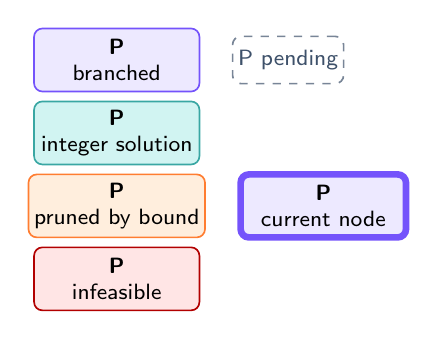
\begin{tikzpicture}[node distance=3pt]
 \node[bbnode,bbbranched] (a) {\textbf{P} \\ branched};
 \node[bbnode,bbinteger,below=of a] (b) {\textbf{P} \\ integer solution};
 \node[bbnode,bbpruned,below=of b] (c) {\textbf{P} \\ pruned by bound};
 \node[bbnode,bbinfeasible,below=of c] (d) {\textbf{P} \\ infeasible};
 \node[bbnode,bbpending,right=0.4cm of a] (e) {P pending};
 \node[bbnode,bbbranched,bbcur,right=0.4cm of c] (f) {\textbf{P} \\ current node};
\end{tikzpicture}
\end{center}
\end{column}
\end{columns}
\end{frame}

\makesection{Problem 1}
\begin{frame}{Problem 1 · Statement}
\noindent{\Large\[\begin{aligned}&\max\ z = 5x_1 + 2x_2\\[4pt] \text{s.t.}\ \ & 3x_1 + x_2 \le 12\\ & x_1 + x_2 \le 5\\ & x_1,x_2\ge 0;\ x_1,x_2\ \text{integer}\end{aligned}\]}
\end{frame}

\begin{frame}{Problem 1 · LINGO: root LP (P1)}
\begin{columns}[T]
\begin{column}{0.40\textwidth}
\colheader{LINGO model}
{\footnotesize \texttt{MAX = 5{*}x1 + 2{*}x2;}\\ \texttt{3{*}x1 + x2 $\le$ 12;}\\ \texttt{x1 + x2 $\le$ 5;}\\ \texttt{END}\par}
\colheader{Result}
{\footnotesize $z=\frac{51}{2}\approx 20.5$,\quad $x_1=\frac{7}{2}\approx3.5$,\quad $x_2=\frac{3}{2}\approx 1.5$\par}\vspace{4pt}
\colheader{Decision}
{\footnotesize $x_1=3.5$ is fractional $\Rightarrow$ branch: \textbf{P2} with $x_1\le 3$ \; and \; \textbf{P3} with $x_1\ge 4$.\par}
\end{column}
\begin{column}{0.58\textwidth}
\lingoshot{p1_P1}
\end{column}
\end{columns}
\end{frame}

\begin{frame}{Problem 1 · Tree after solving P1}
\noindent{\small \textbf{Step 1:} P1 solved (branched). \hfill {\footnotesize Current incumbent: none}\par}
\bbset{1}\bbTreeUno
\end{frame}

\begin{frame}{Problem 1 · Subproblem P2: LINGO}
\begin{columns}[T]
\begin{column}{0.44\textwidth}
\colheader{LINGO model}
{\footnotesize \texttt{MAX = 5{*}x1 + 2{*}x2;}\\ \texttt{3{*}x1 + x2 $\le$ 12;}\\ \texttt{x1 + x2 $\le$ 5;}\\ \texttt{x1 $\le$ 3;}\\ \texttt{END}\par}\vspace{4pt}
\colheader{Result}
{\footnotesize $z=19$,\quad $x_1=3$,\quad $x_2=2$\par}\vspace{4pt}
\colheader{Decision}
{\footnotesize Feasible integer solution $\Rightarrow$ new \textbf{incumbent} $z^*=19$. Node fathomed.\par}
\end{column}
\begin{column}{0.54\textwidth}
\lingoshot{p1_P2}
\end{column}
\end{columns}
\end{frame}

\begin{frame}{Problem 1 · Tree after solving P2}
\noindent{\small \textbf{Step 2:} P2 solved (integer). \hfill {\footnotesize Current incumbent: $z^*=19$ at $(3,2)$}\par}
\bbset{2}\bbTreeUno
\end{frame}

\begin{frame}{Problem 1 · Subproblem P3: LINGO}
\begin{columns}[T]
\begin{column}{0.44\textwidth}
\colheader{LINGO model}
{\footnotesize \texttt{MAX = 5{*}x1 + 2{*}x2;}\\ \texttt{3{*}x1 + x2 $\le$ 12;}\\ \texttt{x1 + x2 $\le$ 5;}\\ \texttt{x1 $\ge$ 4;}\\ \texttt{END}\par}\vspace{4pt}
\colheader{Result}
{\footnotesize $z=20$,\quad $x_1=4$,\quad $x_2=0$\par}\vspace{4pt}
\colheader{Decision}
{\footnotesize Feasible integer solution $\Rightarrow$ new \textbf{incumbent} $z^*=20$. Node fathomed.\par}
\end{column}
\begin{column}{0.54\textwidth}
\lingoshot{p1_P3}
\end{column}
\end{columns}
\end{frame}

\begin{frame}{Problem 1 · Tree after solving P3}
\noindent{\small \textbf{Step 3:} P3 solved (integer). \hfill {\footnotesize Current incumbent: $z^*=20$ at $(4,0)$}\par}
\bbset{3}\bbTreeUno
\end{frame}

\begin{frame}{Problem 1 · Final solution}
\noindent{\small \textbf{Optimal solution:} $z^*=20$,\ $x_1^*=4$,\ $x_2^*=0$ \hfill (3 subproblems solved)\par}
\bbset{99}\bbTreeUno
\end{frame}

\makesection{Problem 3}
\begin{frame}{Problem 3 · Statement}
\noindent{\Large\[\begin{aligned}&\max\ z = 2x_1 + 3x_2\\[4pt] \text{s.t.}\ \ & x_1 + 2x_2 \le 10\\ & 3x_1 + 4x_2 \le 25\\ & x_1,x_2\ge 0;\ x_1,x_2\ \text{integer}\end{aligned}\]}
\end{frame}

\begin{frame}{Problem 3 · LINGO: root LP (P1)}
\begin{columns}[T]
\begin{column}{0.40\textwidth}
\colheader{LINGO model}
{\footnotesize \texttt{MAX = 2{*}x1 + 3{*}x2;}\\ \texttt{x1 + 2{*}x2 $\le$ 10;}\\ \texttt{3{*}x1 + 4{*}x2 $\le$ 25;}\\ \texttt{END}\par}
\colheader{Result}
{\footnotesize $z=\frac{35}{2}\approx 17.5$,\quad $x_1=5$,\quad $x_2=\frac{5}{2}\approx 2.5$\par}\vspace{4pt}
\colheader{Decision}
{\footnotesize $x_2=\frac{5}{2}\approx 2.5$ is fractional $\Rightarrow$ branch: \textbf{P2} with $x_2\le 2$ \; and \; \textbf{P3} with $x_2\ge 3$.\par}
\end{column}
\begin{column}{0.58\textwidth}
\lingoshot{p3_P1}
\end{column}
\end{columns}
\end{frame}

\begin{frame}{Problem 3 · Tree after solving P1}
\noindent{\small \textbf{Step 1:} P1 solved (branched). \hfill {\footnotesize Current incumbent: none}\par}
\bbset{1}\bbTreeTres
\end{frame}

\begin{frame}{Problem 3 · Subproblem P2: LINGO}
\begin{columns}[T]
\begin{column}{0.44\textwidth}
\colheader{LINGO model}
{\footnotesize \texttt{MAX = 2{*}x1 + 3{*}x2;}\\ \texttt{x1 + 2{*}x2 $\le$ 10;}\\ \texttt{3{*}x1 + 4{*}x2 $\le$ 25;}\\ \texttt{x2 $\le$ 2;}\\ \texttt{END}\par}\vspace{4pt}
\colheader{Result}
{\footnotesize $z=\frac{52}{3}\approx 17.33$,\quad $x_1=\frac{17}{3}\approx 5.66$,\quad $x_2=2$\par}\vspace{4pt}
\colheader{Decision}
{\footnotesize $x_1=\frac{17}{3}\approx 5.66$ is fractional $\Rightarrow$ branch: \textbf{P4} with $x_1\le 5$ \; and \; \textbf{P5} with $x_1\ge 6$.\par}
\end{column}
\begin{column}{0.54\textwidth}
\lingoshot{p3_P2}
\end{column}
\end{columns}
\end{frame}

\begin{frame}{Problem 3 · Tree after solving P2}
\noindent{\small \textbf{Step 2:} P2 solved (branched). \hfill {\footnotesize Current incumbent: none}\par}
\bbset{2}\bbTreeTres
\end{frame}

\begin{frame}{Problem 3 · Subproblem P4: LINGO}
\begin{columns}[T]
\begin{column}{0.44\textwidth}
\colheader{LINGO model}
{\footnotesize \texttt{MAX = 2{*}x1 + 3{*}x2;}\\ \texttt{x1 + 2{*}x2 $\le$ 10;}\\ \texttt{3{*}x1 + 4{*}x2 $\le$ 25;}\\ \texttt{x1 $\le$ 5;}\\ \texttt{END}\par}\vspace{4pt}
\colheader{Result}
{\footnotesize $z=\frac{35}{2}\approx 17.5$,\quad $x_1=5$,\quad $x_2=\frac{5}{2}\approx 2.5$\par}\vspace{4pt}
\colheader{Decision}
{\footnotesize Subproblem \textbf{P4} is the same as \textbf{P1}, so it gets pruned, because it is a repeated subproblem.\par}
\end{column}
\begin{column}{0.54\textwidth}
\lingoshot{p3_P4}
\end{column}
\end{columns}
\end{frame}

\begin{frame}{Problem 3 · Tree after solving P4}
\noindent{\small \textbf{Step 3:} P4 solved (pruned). \hfill {\footnotesize Current incumbent: none}\par}
\bbset{3}\bbTreeTres
\end{frame}

\begin{frame}{Problem 3 · Subproblem P5: LINGO}
\begin{columns}[T]
\begin{column}{0.44\textwidth}
\colheader{LINGO model}
{\footnotesize \texttt{MAX = 2{*}x1 + 3{*}x2;}\\ \texttt{x1 + 2{*}x2 $\le$ 10;}\\ \texttt{3{*}x1 + 4{*}x2 $\le$ 25;}\\ \texttt{x1 $\ge$ 6;}\\ \texttt{END}\par}\vspace{4pt}
\colheader{Result}
{\footnotesize $z=\frac{69}{4}\approx 17.25$,\quad $x_1=6$,\quad $x_2=\frac{7}{4}\approx 1.75$\par}\vspace{4pt}
\colheader{Decision}
{\footnotesize $x_2=\frac{7}{4}\approx 1.75$ is fractional $\Rightarrow$ branch: \textbf{P6} with $x_2\le 1$ \; and \; \textbf{P7} with $x_2\ge 2$.\par}
\end{column}
\begin{column}{0.54\textwidth}
\lingoshot{p3_P5}
\end{column}
\end{columns}
\end{frame}

\begin{frame}{Problem 3 · Tree after solving P5}
\noindent{\small \textbf{Step 4:} P5 solved (branched). \hfill {\footnotesize Current incumbent: none}\par}
\bbset{4}\bbTreeTres
\end{frame}

\begin{frame}{Problem 3 · Subproblem P6: LINGO}
\begin{columns}[T]
\begin{column}{0.44\textwidth}
\colheader{LINGO model}
{\footnotesize \texttt{MAX = 2{*}x1 + 3{*}x2;}\\ \texttt{x1 + 2{*}x2 $\le$ 10;}\\ \texttt{3{*}x1 + 4{*}x2 $\le$ 25;}\\ \texttt{x2 $\le$ 1;}\\ \texttt{END}\par}\vspace{4pt}
\colheader{Result}
{\footnotesize $z=17$,\quad $x_1=7$,\quad $x_2=1$\par}\vspace{4pt}
\colheader{Decision}
{\footnotesize Feasible integer solution $\Rightarrow$ new \textbf{incumbent} $z^*=17$. Node fathomed.\par}
\end{column}
\begin{column}{0.54\textwidth}
\lingoshot{p3_P6}
\end{column}
\end{columns}
\end{frame}

\begin{frame}{Problem 3 · Tree after solving P6}
\noindent{\small \textbf{Step 5:} P6 solved (integer). \hfill {\footnotesize Current incumbent: $z^*=17$ at $(7,1)$}\par}
\bbset{5}\bbTreeTres
\end{frame}

\begin{frame}{Problem 3 · Subproblem P7: LINGO}
\begin{columns}[T]
\begin{column}{0.44\textwidth}
\colheader{LINGO model}
{\footnotesize \texttt{MAX = 2{*}x1 + 3{*}x2;}\\ \texttt{x1 + 2{*}x2 $\le$ 10;}\\ \texttt{3{*}x1 + 4{*}x2 $\le$ 25;}\\ \texttt{x2 $\ge$ 2;}\\ \texttt{END}\par}\vspace{4pt}
\colheader{Result}
{\footnotesize $z=\frac{35}{2}\approx 17.5$,\quad $x_1=5$,\quad $x_2=\frac{5}{2}\approx 2.5$\par}\vspace{4pt}
\colheader{Decision}
{\footnotesize Subproblem \textbf{P7} is the same as \textbf{P1}, so it gets pruned, because it is a repeated subproblem.\par}
\end{column}
\begin{column}{0.54\textwidth}
\lingoshot{p3_P7}
\end{column}
\end{columns}
\end{frame}

\begin{frame}{Problem 3 · Tree after solving P7}
\noindent{\small \textbf{Step 6:} P7 solved (pruned). \hfill {\footnotesize Current incumbent: $z^*=17$ at $(7,1)$}\par}
\bbset{6}\bbTreeTres
\end{frame}

\begin{frame}{Problem 3 · Subproblem P3: LINGO}
\begin{columns}[T]
\begin{column}{0.44\textwidth}
\colheader{LINGO model}
{\footnotesize \texttt{MAX = 2{*}x1 + 3{*}x2;}\\ \texttt{x1 + 2{*}x2 $\le$ 10;}\\ \texttt{3{*}x1 + 4{*}x2 $\le$ 25;}\\ \texttt{x2 $\ge$ 3;}\\ \texttt{END}\par}\vspace{4pt}
\colheader{Result}
{\footnotesize $z=17$,\quad $x_1=4$,\quad $x_2=3$\par}\vspace{4pt}
\colheader{Decision}
{\footnotesize Feasible integer solution, but the current incumbent solution has the same $Z$ value.\par}
\end{column}
\begin{column}{0.54\textwidth}
\lingoshot{p3_P7}
\end{column}
\end{columns}
\end{frame}

\begin{frame}{Problem 3 · Tree after solving P3}
\noindent{\small \textbf{Step 6:} P3 solved (pruned). \hfill {\footnotesize Current incumbent: $z^*=17$ at $(7,1)$}\par}
\bbset{7}\bbTreeTres
\end{frame}

\begin{frame}{Problem 3 · Final solution}
\noindent{\small \textbf{Optimal solution:} $z^*=17$,\ $x_1^*=7$,\ $x_2^*=1$ \hfill (7 subproblems solved)\par}
\bbset{99}\bbTreeTres
\end{frame}

\makesection{Problem 4}
\begin{frame}{Problem 4 · Statement}
\noindent{\Large\[\begin{aligned}&\max\ z = 4x_1 + 3x_2\\[4pt] \text{s.t.}\ \ & 4x_1 + 9x_2 \le 26\\ & 8x_1 + 5x_2 \le 17\\ & x_1,x_2\ge 0;\ x_1,x_2\ \text{integer}\end{aligned}\]}
\end{frame}

\begin{frame}{Problem 4 · LINGO: root LP (P1)}
\begin{columns}[T]
\begin{column}{0.40\textwidth}
\colheader{LINGO model}
{\footnotesize \texttt{MAX = 4{*}x1 + 3{*}x2;}\\ \texttt{4{*}x1 + 9{*}x2 $\le$ 26;}\\ \texttt{8{*}x1 + 5{*}x2 $\le$ 17;}\\ \texttt{END}\par}
\end{column}
\begin{column}{0.58\textwidth}
\lingoshot{p4_P1}
\end{column}
\end{columns}
\end{frame}

\makesection{Problem 5}
\begin{frame}{Problem 5 · Statement}
\noindent{\Large\[\begin{aligned}&\max\ z = 4x_1 + 5x_2\\[4pt] \text{s.t.}\ \ & x_1 + 4x_2 \ge 5\\ & 3x_1 + 2x_2 \ge 7\\ & x_1,x_2\ge 0;\ x_1,x_2\ \text{integer}\end{aligned}\]}
\end{frame}

\begin{frame}{Problem 5 · LINGO: root LP (P1)}
\begin{columns}[T]
\begin{column}{0.40\textwidth}
\colheader{LINGO model}
{\footnotesize \texttt{MAX = 4{*}x1 + 5{*}x2;}\\ \texttt{x1 + 4{*}x2 $\ge$ 5;}\\ \texttt{3{*}x1 + 2{*}x2 $\ge$ 7;}\\ \texttt{END}\par}
\end{column}
\begin{column}{0.58\textwidth}
\lingoshot{p5_P1}
\end{column}
\end{columns}
\end{frame}

\makesection{Problem 6}
\begin{frame}{Problem 6 · Statement}
\noindent{\Large\[\begin{aligned}&\max\ z = 4x_1 + 5x_2\\[4pt] \text{s.t.}\ \ & 3x_1 + 2x_2 \le 10\\ & x_1 + 4x_2 \le 11\\ & 3x_1 + 3x_2 \le 13\\ & x_1,x_2\ge 0;\ x_1,x_2\ \text{integer}\end{aligned}\]}
\end{frame}

\begin{frame}{Problem 6 · Subproblem P1: LINGO}
\begin{columns}[T]
\begin{column}{0.44\textwidth}
\colheader{LINGO model}
{\footnotesize \texttt{MAX = 4{*}x1 + 5{*}x2;}\\ \texttt{3{*}x1 + 2{*}x2 $\le$ 10;}\\ \texttt{x1 + 4{*}x2 $\le$ 11;}\\ \texttt{3{*}x1 + 3{*}x2 $\le$ 13;}\\ \texttt{END}\par}\vspace{4pt}
\colheader{Result}
{\footnotesize $z=\frac{187}{10}\approx 18.7$,\quad $x_1=\frac{9}{5}\approx 1.8$,\quad $x_2=\frac{23}{10}\approx 2.3$\par}\vspace{4pt}
\colheader{Decision}
{\footnotesize $x_1=\frac{9}{5}$ is fractional $\Rightarrow$ branch: \textbf{P2} with $x_1\le 1$ \; and \; \textbf{P3} with $x_1\ge 2$.\par}
\end{column}
\begin{column}{0.54\textwidth}
\lingoshot{p6_P1}
\end{column}
\end{columns}
\end{frame}

\begin{frame}{Problem 6 · Tree after solving P1}
\noindent{\small \textbf{Step 1:} P1 solved (branched). \hfill {\footnotesize Current incumbent: none}\par}
\bbset{1}\bbTreeSeis
\end{frame}

\begin{frame}{Problem 6 · Subproblem P2: LINGO}
\begin{columns}[T]
\begin{column}{0.44\textwidth}
\colheader{LINGO model}
{\footnotesize \texttt{MAX = 4{*}x1 + 5{*}x2;}\\ \texttt{3{*}x1 + 2{*}x2 $\le$ 10;}\\ \texttt{x1 + 4{*}x2 $\le$ 11;}\\ \texttt{3{*}x1 + 3{*}x2 $\le$ 13;}\\ \texttt{x1 $\le$ 1;}\\ \texttt{END}\par}\vspace{4pt}
\colheader{Result}
{\footnotesize $z=\frac{33}{2}\approx 16.5$,\quad $x_1=1$,\quad $x_2=\frac{5}{2}\approx 2.5$\par}\vspace{4pt}
\colheader{Decision}
{\footnotesize $x_2=\frac{5}{2}$ is fractional $\Rightarrow$ branch: \textbf{P4} with $x_2\le 2$ \; and \; \textbf{P5} with $x_2\ge 3$.\par}
\end{column}
\begin{column}{0.54\textwidth}
\lingoshot{p6_P2}
\end{column}
\end{columns}
\end{frame}

\begin{frame}{Problem 6 · Tree after solving P2}
\noindent{\small \textbf{Step 2:} P2 solved (branched). \hfill {\footnotesize Current incumbent: none}\par}
\bbset{2}\bbTreeSeis
\end{frame}

\begin{frame}{Problem 6 · Subproblem P4: LINGO}
\begin{columns}[T]
\begin{column}{0.44\textwidth}
\colheader{LINGO model}
{\footnotesize \texttt{MAX = 4{*}x1 + 5{*}x2;}\\ \texttt{3{*}x1 + 2{*}x2 $\le$ 10;}\\ \texttt{x1 + 4{*}x2 $\le$ 11;}\\ \texttt{3{*}x1 + 3{*}x2 $\le$ 13;}\\ \texttt{x1 $\le$ 1;}\\ \texttt{x2 $\le$ 2;}\\ \texttt{END}\par}\vspace{4pt}
\colheader{Result}
{\footnotesize $z=14$,\quad $x_1=1$,\quad $x_2=2$\par}\vspace{4pt}
\colheader{Decision}
{\footnotesize Feasible integer solution $\Rightarrow$ new \textbf{incumbent} $z^*=14$. Node fathomed.\par}
\end{column}
\begin{column}{0.54\textwidth}
\lingoshot{p6_P4}
\end{column}
\end{columns}
\end{frame}

\begin{frame}{Problem 6 · Tree after solving P4}
\noindent{\small \textbf{Step 3:} P4 solved (integer). \hfill {\footnotesize Current incumbent: $z^*=14$ at $(1,2)$}\par}
\bbset{3}\bbTreeSeis
\end{frame}

\begin{frame}{Problem 6 · Subproblem P5: LINGO}
\begin{columns}[T]
\begin{column}{0.44\textwidth}
\colheader{LINGO model}
{\footnotesize \texttt{MAX = 4{*}x1 + 5{*}x2;}\\ \texttt{3{*}x1 + 2{*}x2 $\le$ 10;}\\ \texttt{x1 + 4{*}x2 $\le$ 11;}\\ \texttt{3{*}x1 + 3{*}x2 $\le$ 13;}\\ \texttt{x1 $\le$ 1;}\\ \texttt{x2 $\ge$ 3;}\\ \texttt{END}\par}\vspace{4pt}
\colheader{Result}
{\footnotesize LINGO reports: \textbf{Infeasible}\par}\vspace{4pt}
\colheader{Decision}
{\footnotesize Empty feasible region $\Rightarrow$ node fathomed by \textbf{infeasibility}.\par}
\end{column}
\begin{column}{0.54\textwidth}
\lingoshot{p6_P5}
\end{column}
\end{columns}
\end{frame}

\begin{frame}{Problem 6 · Tree after solving P5}
\noindent{\small \textbf{Step 4:} P5 solved (infeasible). \hfill {\footnotesize Current incumbent: $z^*=14$ at $(1,2)$}\par}
\bbset{4}\bbTreeSeis
\end{frame}

\begin{frame}{Problem 6 · Subproblem P3: LINGO}
\begin{columns}[T]
\begin{column}{0.44\textwidth}
\colheader{LINGO model}
{\footnotesize \texttt{MAX = 4{*}x1 + 5{*}x2;}\\ \texttt{3{*}x1 + 2{*}x2 $\le$ 10;}\\ \texttt{x1 + 4{*}x2 $\le$ 11;}\\ \texttt{3{*}x1 + 3{*}x2 $\le$ 13;}\\ \texttt{x1 $\ge$ 2;}\\ \texttt{END}\par}\vspace{4pt}
\colheader{Result}
{\footnotesize $z=18$,\quad $x_1=2$,\quad $x_2=2$\par}\vspace{4pt}
\colheader{Decision}
{\footnotesize Feasible integer solution $\Rightarrow$ new \textbf{incumbent} $z^*=18$. Node fathomed.\par}
\end{column}
\begin{column}{0.54\textwidth}
\lingoshot{p6_P3}
\end{column}
\end{columns}
\end{frame}

\begin{frame}{Problem 6 · Tree after solving P3}
\noindent{\small \textbf{Step 5:} P3 solved (integer). \hfill {\footnotesize Current incumbent: $z^*=18$ at $(2,2)$}\par}
\bbset{5}\bbTreeSeis
\end{frame}

\begin{frame}{Problem 6 · Final solution}
\noindent{\small \textbf{Optimal solution:} $z^*=18$,\ $x_1^*=2$,\ $x_2^*=2$ \hfill (5 subproblems solved)\par}
\bbset{99}\bbTreeSeis
\end{frame}

\makesection{Problem 7}
\begin{frame}{Problem 7 · Statement}
\noindent{\Large\[\begin{aligned}&\max\ z = 7x_1 + 3x_2\\[4pt] \text{s.t.}\ \ & 2x_1 + x_2 \le 9\\ & 3x_1 + 2x_2 \le 13\\ & x_1,x_2\ge 0;\ x_1,x_2\ \text{integer}\end{aligned}\]}
\end{frame}

\begin{frame}{Problem 7 · Subproblem P1: LINGO}
\begin{columns}[T]
\begin{column}{0.44\textwidth}
\colheader{LINGO model}
{\footnotesize \texttt{MAX = 7{*}x1 + 3{*}x2;}\\ \texttt{2{*}x1 + x2 $\le$ 9;}\\ \texttt{3{*}x1 + 2{*}x2 $\le$ 13;}\\ \texttt{END}\par}\vspace{4pt}
\colheader{Result}
{\footnotesize $z=\frac{91}{3}\approx 30.33$,\quad $x_1=\frac{13}{3}\approx 4.33$,\quad $x_2=0$\par}\vspace{4pt}
\colheader{Decision}
{\footnotesize $x_1=\frac{13}{3}$ is fractional $\Rightarrow$ branch: \textbf{P2} with $x_1\le 4$ \; and \; \textbf{P3} with $x_1\ge 5$.\par}
\end{column}
\begin{column}{0.54\textwidth}
\lingoshot{p7_P1}
\end{column}
\end{columns}
\end{frame}

\begin{frame}{Problem 7 · Tree after solving P1}
\noindent{\small \textbf{Step 1:} P1 solved (branched). \hfill {\footnotesize Current incumbent: none}\par}
\bbset{1}\bbTreeSiete
\end{frame}

\begin{frame}{Problem 7 · Subproblem P2: LINGO}
\begin{columns}[T]
\begin{column}{0.44\textwidth}
\colheader{LINGO model}
{\footnotesize \texttt{MAX = 7{*}x1 + 3{*}x2;}\\ \texttt{2{*}x1 + x2 $\le$ 9;}\\ \texttt{3{*}x1 + 2{*}x2 $\le$ 13;}\\ \texttt{x1 $\le$ 4;}\\ \texttt{END}\par}\vspace{4pt}
\colheader{Result}
{\footnotesize $z=\frac{59}{2}\approx 29.5$,\quad $x_1=4$,\quad $x_2=\frac{1}{2}\approx 0.5$\par}\vspace{4pt}
\colheader{Decision}
{\footnotesize $x_2=\frac{1}{2}$ is fractional $\Rightarrow$ branch: \textbf{P4} with $x_2\le 0$ \; and \; \textbf{P5} with $x_2\ge 1$.\par}
\end{column}
\begin{column}{0.54\textwidth}
\lingoshot{p7_P2}
\end{column}
\end{columns}
\end{frame}

\begin{frame}{Problem 7 · Tree after solving P2}
\noindent{\small \textbf{Step 2:} P2 solved (branched). \hfill {\footnotesize Current incumbent: none}\par}
\bbset{2}\bbTreeSiete
\end{frame}

\begin{frame}{Problem 7 · Subproblem P4: LINGO}
\begin{columns}[T]
\begin{column}{0.44\textwidth}
\colheader{LINGO model}
{\footnotesize \texttt{MAX = 7{*}x1 + 3{*}x2;}\\ \texttt{2{*}x1 + x2 $\le$ 9;}\\ \texttt{3{*}x1 + 2{*}x2 $\le$ 13;}\\ \texttt{x1 $\le$ 4;}\\ \texttt{x2 $\le$ 0;}\\ \texttt{END}\par}\vspace{4pt}
\colheader{Result}
{\footnotesize $z=28$,\quad $x_1=4$,\quad $x_2=0$\par}\vspace{4pt}
\colheader{Decision}
{\footnotesize Feasible integer solution $\Rightarrow$ new \textbf{incumbent} $z^*=28$. Node fathomed.\par}
\end{column}
\begin{column}{0.54\textwidth}
\lingoshot{p7_P4}
\end{column}
\end{columns}
\end{frame}

\begin{frame}{Problem 7 · Tree after solving P4}
\noindent{\small \textbf{Step 3:} P4 solved (integer). \hfill {\footnotesize Current incumbent: $z^*=28$ at $(4,0)$}\par}
\bbset{3}\bbTreeSiete
\end{frame}

\begin{frame}{Problem 7 · Subproblem P5: LINGO}
\begin{columns}[T]
\begin{column}{0.44\textwidth}
\colheader{LINGO model}
{\footnotesize \texttt{MAX = 7{*}x1 + 3{*}x2;}\\ \texttt{2{*}x1 + x2 $\le$ 9;}\\ \texttt{3{*}x1 + 2{*}x2 $\le$ 13;}\\ \texttt{x1 $\le$ 4;}\\ \texttt{x2 $\ge$ 1;}\\ \texttt{END}\par}\vspace{4pt}
\colheader{Result}
{\footnotesize $z=\frac{86}{3}\approx 28.67$,\quad $x_1=\frac{11}{3}\approx 3.67$,\quad $x_2=1$\par}\vspace{4pt}
\colheader{Decision}
{\footnotesize $x_1=\frac{11}{3}$ is fractional $\Rightarrow$ branch: \textbf{P6} with $x_1\le 3$ \; and \; \textbf{P7} with $x_1\ge 4$.\par}
\end{column}
\begin{column}{0.54\textwidth}
\lingoshot{p7_P5}
\end{column}
\end{columns}
\end{frame}

\begin{frame}{Problem 7 · Tree after solving P5}
\noindent{\small \textbf{Step 4:} P5 solved (branched). \hfill {\footnotesize Current incumbent: $z^*=28$ at $(4,0)$}\par}
\bbset{4}\bbTreeSiete
\end{frame}

\begin{frame}{Problem 7 · Subproblem P6: LINGO}
\begin{columns}[T]
\begin{column}{0.44\textwidth}
\colheader{LINGO model}
{\footnotesize \texttt{MAX = 7{*}x1 + 3{*}x2;}\\ \texttt{2{*}x1 + x2 $\le$ 9;}\\ \texttt{3{*}x1 + 2{*}x2 $\le$ 13;}\\ \texttt{x1 $\le$ 3;}\\ \texttt{x2 $\ge$ 1;}\\ \texttt{END}\par}\vspace{4pt}
\colheader{Result}
{\footnotesize $z=27$,\quad $x_1=3$,\quad $x_2=2$\par}\vspace{4pt}
\colheader{Decision}
{\footnotesize $z=27$ does not improve the incumbent $z^*=28$ ($\le$) $\Rightarrow$ pruned by \textbf{bound} (the solution is integer but not better).\par}
\end{column}
\begin{column}{0.54\textwidth}
\lingoshot{p7_P6}
\end{column}
\end{columns}
\end{frame}

\begin{frame}{Problem 7 · Tree after solving P6}
\noindent{\small \textbf{Step 5:} P6 solved (pruned). \hfill {\footnotesize Current incumbent: $z^*=28$ at $(4,0)$}\par}
\bbset{5}\bbTreeSiete
\end{frame}

\begin{frame}{Problem 7 · Subproblem P7: LINGO}
\begin{columns}[T]
\begin{column}{0.44\textwidth}
\colheader{LINGO model}
{\footnotesize \texttt{MAX = 7{*}x1 + 3{*}x2;}\\ \texttt{2{*}x1 + x2 $\le$ 9;}\\ \texttt{3{*}x1 + 2{*}x2 $\le$ 13;}\\ \texttt{x1 $\le$ 4;}\\ \texttt{x2 $\ge$ 1;}\\ \texttt{x1 $\ge$ 4;}\\ \texttt{END}\par}\vspace{4pt}
\colheader{Result}
{\footnotesize LINGO reports: \textbf{Infeasible}\par}\vspace{4pt}
\colheader{Decision}
{\footnotesize Empty feasible region $\Rightarrow$ node fathomed by \textbf{infeasibility}.\par}
\end{column}
\begin{column}{0.54\textwidth}
\lingoshot{p7_P7}
\end{column}
\end{columns}
\end{frame}

\begin{frame}{Problem 7 · Tree after solving P7}
\noindent{\small \textbf{Step 6:} P7 solved (infeasible). \hfill {\footnotesize Current incumbent: $z^*=28$ at $(4,0)$}\par}
\bbset{6}\bbTreeSiete
\end{frame}

\begin{frame}{Problem 7 · Subproblem P3: LINGO}
\begin{columns}[T]
\begin{column}{0.44\textwidth}
\colheader{LINGO model}
{\footnotesize \texttt{MAX = 7{*}x1 + 3{*}x2;}\\ \texttt{2{*}x1 + x2 $\le$ 9;}\\ \texttt{3{*}x1 + 2{*}x2 $\le$ 13;}\\ \texttt{x1 $\ge$ 5;}\\ \texttt{END}\par}\vspace{4pt}
\colheader{Result}
{\footnotesize LINGO reports: \textbf{Infeasible}\par}\vspace{4pt}
\colheader{Decision}
{\footnotesize Empty feasible region $\Rightarrow$ node fathomed by \textbf{infeasibility}.\par}
\end{column}
\begin{column}{0.54\textwidth}
\lingoshot{p7_P3}
\end{column}
\end{columns}
\end{frame}

\begin{frame}{Problem 7 · Tree after solving P3}
\noindent{\small \textbf{Step 7:} P3 solved (infeasible). \hfill {\footnotesize Current incumbent: $z^*=28$ at $(4,0)$}\par}
\bbset{7}\bbTreeSiete
\end{frame}

\begin{frame}{Problem 7 · Final solution}
\noindent{\small \textbf{Optimal solution:} $z^*=28$,\ $x_1^*=4$,\ $x_2^*=0$ \hfill (7 subproblems solved)\par}
\bbset{99}\bbTreeSiete
\end{frame}


\makesection{Summary}
\begin{frame}{Summary of results}
\centering\renewcommand{\arraystretch}{1.25}
\begin{tabular}{lcccc}
\toprule
Problem & Objective & Subproblems & $z^*$ & $(x_1^*,x_2^*)$ \\
\midrule
Problem 1 & $\max$ & 3 & $20$ & $(4,\,0)$ \\
Problem 3 & $\max$ & 7 & $17$ & $(7,\,1)$ \\
Problem 4 & $\max$ & 0 & $0$ & $(0,\,0)$ \\
Problem 5 & $\max$ & 0 & $0$ & $(0,\,0)$ \\
Problem 6 & $\max$ & 5 & $18$ & $(2,\,2)$ \\
Problem 7 & $\max$ & 7 & $28$ & $(4,\,0)$ \\
\bottomrule
\end{tabular}
\end{frame}


% =====================================================================
%  TEMPLATE TO ADD A NEW TREE (copy, uncomment, edit)
% =====================================================================
% \newcommand{\bbTreeEjemplo}{%
% \begin{bbtree}
%   \useasboundingbox (-1.4,-4.2) rectangle (6.4,0.8);   % fixed box so the tree does not jump
%   \bbNode{n1}{2.5,0}   {1}{1}{branched}  {P1}{$z{=}20.5$\\$(3.5,\,1.5)$}
%   \bbNode{n2}{0,-1.65} {1}{2}{integer}   {P2}{$z{=}19$\\$(3,\,2)$}
%   \bbNode{n3}{5,-1.65} {1}{3}{integer}   {P3}{$z{=}20$\\$(4,\,0)$}
%   \bbEdge{n1}{n2}{1}{$x_1\le 3$}{left}
%   \bbEdge{n1}{n3}{1}{$x_1\ge 4$}{right}
% \end{bbtree}}
% \begin{frame}{Example: tree at step 2}\bbset{2}\bbTreeEjemplo\end{frame}

\makefinalpage
\finalpagetext{Thank you!}
\end{document}